\section{Types of network machine learning problems}
\label{sec:ch1:types}


There are many different types of network machine learning systems. We tend to broadly group them into the following categories:
\begin{itemize}
\item whether or not they involve one or multiple networks (single or multiple network learning systems),
\item whether or not they require additional information in the form of network attributes (attributed or non-attributed network learning systems),
\item whether they ask questions about an edge, a node, a group of edges/nodes, or about the network itself, and
\item whether or not the approach can be used in isolation from a statistical model (non-model based or model-based network learning systems).

\end{itemize}

To learn about these criteria, we'll use a few running examples:

\begin{floatingbox}[h]\caption{Brain networks for musicians and non-musicians}
\label{box:ch1:brainnet}
You have brain networks that were acquired from a large group of people. The nodes of this network represent areas of the brain, and the edges represent whether a pair of brain areas can communicate using neurons. Neurons are cells in the brain that receive sensory input from the environment, and work together to transform the sensory input into usable outputs (thoughts, actions, behaviors, etc.) Each brain network is from a person who we know is either a non-musician or a musician.
\end{floatingbox}

\begin{floatingbox}[h]\caption{A pair of social networks for students at a school}
\label{box:ch1:social}
In this network, the nodes represent students who attend one of two schools. Edges represent whether the students are connected on a social media site. We have networks collected from two social media sites, Facebook and Twitter.
\end{floatingbox}

\subsection{Single vs multiple network learning systems}

\subsubsection{Single network learning systems}

In many cases of network learning, you only actually have a single sample: the network itself. A \textit{single network learning system} is a system in which insight is derived from a single network, that is one collection of nodes and edges. In a single network learning system, you only have one sample: the network itself. In a traditional machine learning framework, having a single sample is disastrous: you canot derive insight with one sample in a traditional machine learning framework, because a question cannot be addressed using only one data point. This is an extreme case of the small sample problem. As an example, if you wanted to determine the degree to which cloud cover predicted whether or not it was raining, and you only had one day's worth of data, you would not be able to learn anything, because your answer would totally be determined by whether or not it was cloudy on that particular day and whether or not it was raining on that particular day.

On the other hand, in network learning, a single sample is far from disastrous. While we only have one network, that one network is defined by a collection of nodes and edges. For this to be meaningful, there must be multiple nodes and edges in the first place! While you might only have one network, you can still learn about relationships that exist among the nodes, edges, or both. The caveat is that the conclusions you reach from your network might be limited to the specific network you are studying, or a rather limited sample population, but often that’s not much of a problem.


Most of the strategies in this book address single network learning systems.


\subsubsection{Multiple network learning systems}

A \textit{multiple network learning system} is a system in which insight is derived from multiple networks, wherein you have multiple collections of nodes and edges. Unlike a single network learning system in which you can only obtain conclusions on the basis of characteristics of that particular network itself, in a multiple network learning system, you can obtain insights {both} within and across the networks.


In the brain networks from Example \ref{box:ch1:brainnet}, you can derive insights to describe the commonalities among the brain networks of non-musicians along with the commonalities among the brains of musicians, and then compare them to look for differences between the brain networks of non-musicians and musicians.


Some strategies which employ multiple network learning systems are:
\begin{itemize}
\item multiple network representation learning in Section \ref{sec:ch6:multinet},
\item anomaly detection in Section \ref{sec:ch9:anomaly}, and
\item signal subnetworks in Section \ref{sec:ch9:ssn_incoherent}.
\end{itemize}

Note that these these categories are not mutually exclusive, and a network machine learning system will pull elements from several of the different categories simultaneously. For instance, you might have a machine learning system that is a single network, node-attributed, non-model-based machine learning system like a community detection algorithm.

\subsection{Non-attributed vs richly-attributed network learning systems}

In machine learning, you are probably familiar with the terms unsupervised and supervised learning. In network learning, we tend to use a more specific name for these two ideas.


\subsubsection{Non-attributed network learning systems}

The concept of a non-attributed network learning system is directly analogous to the concept of fully unsupervised machine learning. \textit{Unsupervised learning} can be loosely defined as a learning problem in which the data you feed to the algorithm does not include the desired solutions, called \textit{labels}. We call a network learning system \textit{non-attributed} if at the time of analysis, the network(s) you feed your algorithm includes only nodes and edges.


For instance, let's consider the Facebook network from Example \ref{box:ch1:social}. Suppose, unfortunately, that you've lost the information about which students attend which school. You hypothesize that there might be two groups of students in the network, called {communities}, and that if a student is in particular community, they tend to be better friends with other students in the same community. You want to see if you can identify these communities programmatically, and perhaps recover the school information for each student. A non-attributed network learning problem is shown in Figure \ref{fig:ch1:nonattr}. Perhaps, the groups of nodes that are heavily connected (indicated by the gray circles) corresponds to the schools that each student attends.

\begin{figure}[h]
\centering
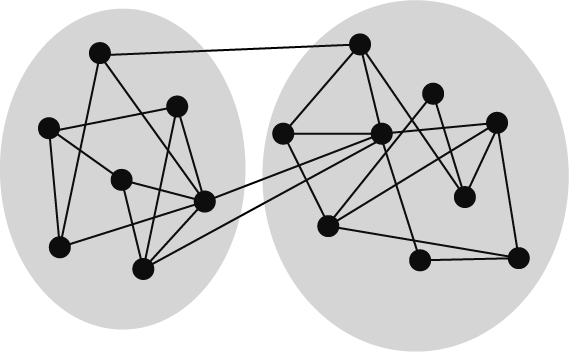
\includegraphics[width=0.5\linewidth]{foundations/ch1/Images/nonattr_ex.png}
\caption[School network hypothesis]{A school network, where the nodes are students and the edges indicate which pairs of students are friends.}
\label{fig:ch1:nonattr}
\end{figure}


Some examples of non-attributed network learning systems are:
\begin{itemize}
\item network embeddings in Section \ref{sec:ch6},
\item community detection in Section \ref{sec:ch7:comm_detect},
\item latent position comparisons in Section \ref{sec:ch8:twosample}, and
\item anomaly detection in Section \ref{sec:ch9:anomaly}.
\end{itemize}


\subsubsection{Attributed network learning systems}

Similarly, the concept of an attributed network learning system is analogous to the concept of supervised or semi-supervised machine learning. \textit{Supervised learning} can be loosely defined as a learning problem in which the data you feed to the algorithm includes {labels}, and \textit{semi-supervised learning} can be loosely defined as a learning problem in which the data you feed to the algorithm includes \textit{some} of the labels. A network is an \textit{attributed network learning system} if at the time of analysis, the network(s) you feed your algorithm include attributes in {addition} to nodes and edges. We have four main types of attributed network learning systems. They are:
\begin{itemize}
\item Networks with node attributes,
\item Networks with edge attributes,
\item Networks with network attributes, and
\item Networks with multiple-network attributes.
\end{itemize}


\paragraph{Networks with node attributes}

A network with \textit{node attributes} is a collection of nodes and edges where, for each node, you have an additional piece of information to describe that node. Let’s consider the school example we talked about above in the section on non-attributed network learning systems. For each student, you also have an additional piece of information: you know which school each student attends, and you want to investigate whether the probability of two students being friends is higher in school one or in school two. A problem for networks with node attributes is shown in Figure \ref{fig:ch1:netnode_edge_attr}(A). 

\begin{figure}[h]
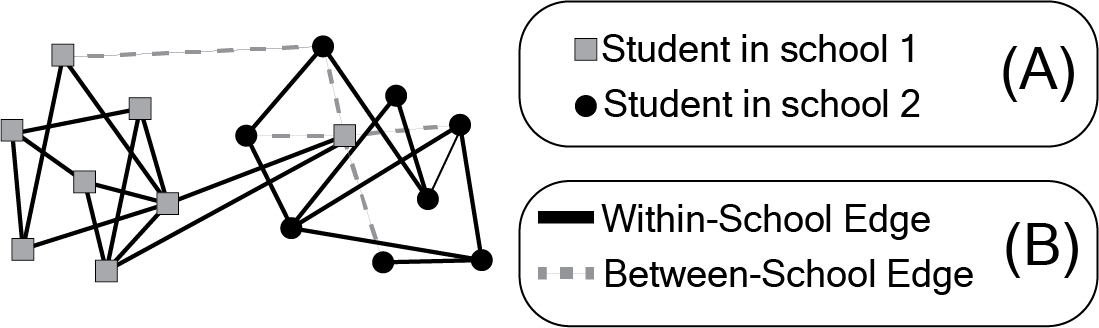
\includegraphics[width=\linewidth]{foundations/ch1/Images/nodeedge_attr.png}
\caption[School with node and edge attributes]{\textbf{(A)} the school network for Facebook, approached using node attributes. \textbf{(B)} the school network for Facebook, approached using edge attributes. Instead of focusing on the school assignments of the nodes, we focus on two groups of edges (the within-school edges, and the between-school edges).}
\label{fig:ch1:netnode_edge_attr}
\end{figure}


Some examples of problems which deal with node attributes are:
\begin{itemize}
\item 

joint representation learning in Section \ref{sec:ch6:joint},

\item 

model selection in Section \ref{sec:ch7:modelselect},

\item 

testing for differences in block matrices in Section \ref{sec:ch8:twosamplesbm}, and

\item 

testing for differences between groups of edges in Section \ref{sec:ch7:testing}.

\end{itemize}

\paragraph{Networks with edge attributes}

A network with edge attributes is a network consisting of nodes and edges where, for each edge, you have an additional piece of information to characterize that edge. For instance, if we return to the Facebook school network from Example \ref{box:ch1:social} that we posed above, we could entirely ignore the school assignments, and simply focus on whether the students have more friends within schools (solid edges) or between schools (dashed edges). This example is shown in Figure \ref{fig:ch1:netnode_edge_attr}(B).


A problem with edge attributes is testing for differences between groups of edges in Section \ref{sec:ch7:testing}.


\paragraph{Networks with network attributes}

A network with network attributes is a collection of networks (each of which has nodes and edges) where, for each network, you have an additional piece of information to characterize that network. Returning to Example \ref{box:ch1:brainnet}, each brain network was from either a musician or a non-musician. This piece of information characterizes each of the networks as either from a musician or a non-musician individual, and applies to the {entire} collection of nodes and edges for a given network. A network with network attributes is shown in Figure \ref{fig:ch1:netnetattr}.

\begin{figure}[h]
\centering
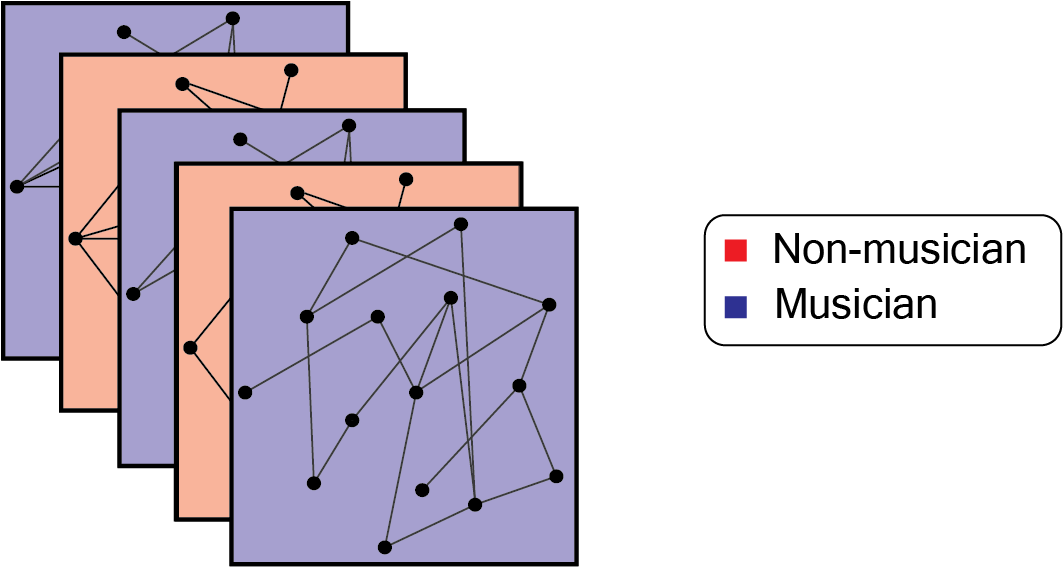
\includegraphics[width=0.8\linewidth]{foundations/ch1/Images/netattr_ex.png}
\caption[Brain networks]{A collection of brain networks, where the nodes are areas of the brain and the edges indicate which brain areas can communicate. For each network, you know whether it comes from a musician or a non-musician.}
\label{fig:ch1:netnetattr}
\end{figure}


An example of a problem which leverages network attributes are signal subgraphs in Section \ref{sec:ch9:ssn_incoherent}.


\paragraph{Networks with multiple-network attributes}

A network with \textit{multiple-network attributes} is a collection of networks (each of which has nodes and edges) where you have additional information that describes how the nodes (or the edges) of the networks relate to one another. Returning to Example \ref{box:ch1:social}, let's add another dimension. The accounts are, for all intents and purposes, anonymous, in that people choose not to share identifying information about themselves on the accounts. However, for three of the people, you know that their two accounts are {matched} together. You want to see if you can use this cross-network attribute (the {matched accounts}) to discover suitable matchings for the remaining accounts in the network. A problem with multiple-network attributes is shown in Figure \ref{fig:ch1:netmultiattr}.

\begin{figure}[h]
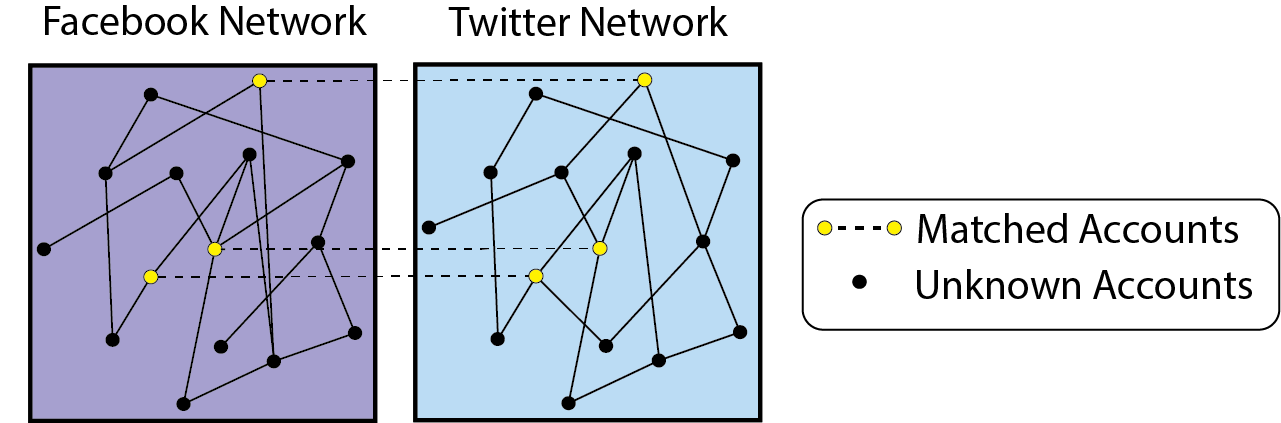
\includegraphics[width=\linewidth]{foundations/ch1/Images/crossnetattr_ex.png}
\caption[Multiple network attributes]{Two social networks from different social media sites. The nodes are people’s accounts on the social media sites (they are the same for both sites) and the edges indicate which pairs of accounts follow one another for that particular site. For three of the people in the network, you know their accounts.}
\label{fig:ch1:netmultiattr}
\end{figure}


An example of problems which leverage cross-network attributes include:
\begin{itemize}
\item Seeded graph matching in Section \ref{sec:ch8:gm}, and
\item Vertex nomination for two networks in Section \ref{sec:ch8:vnviasgm}.
\end{itemize}

\subsection{What part of the network your question is asking about}

In network machine learning, it’s easy to get lost because you're tempted to explore the entire network, whereas your question might be far more limited. For instance, in a transportation network, you might have a collection of nodes representing stations, and a collection of edges representing the number of riders per train during rush hour. You might have a single network for each week of the entire year. We’ll show an example of each type of question from the perspective of the attributes of these networks. 
\begin{enumerate}
    \item Studying a single edge: You might want to know whether a particular edge between two stations could require an additional train because the route is popular during rush hour, and you might only want to study this particular edge over many networks to get some idea of how many passengers take each train.
    \item Studying a single node: You might want to explore the number of passengers who pass through a particular station when deciding whether to approve or reject the expansion of a particular station to include more platforms.
    \item Studying groups of nodes or edges: You might consider cancelling an entire line and need to consider the ramifications of this decision on other stations (groups of nodes) and numbers of passengers per line (groups of edges).
    \item Studying the entire network: You might need to determine whether more funds need to be allocated to public transportation as a whole, and therefore to study how much transportation via the network saves the city over the course of the year.
\end{enumerate}


\subsection{Model-based vs non-model-based network learning systems}

Statistics tends to form somewhat of a ``core'' to network learning systems. This is because in any network learning problem, there is always room for randomness, whether it comes in the form of the particulars of the network you sampled, the set of networks you acquired, the nature of the data you collected, or many other factors. 

We will provide a more rigorous definition later, but for now, you can understand a \textit{statistical model} to be a conceptual framework of a problem that allows you to explicitly account for variation, randomness, or error in your sample (the data you actually obtain) compared to the entirety of the actual object or set of objects that you are studying (the \textit{population}). This balance between model-based and non-model-based network learning is a core aim of this book, so we do not expect you to be able to conceptualize the difference just yet. For this reason, we will try to explain the difference without talking about networks for now.


\subsubsection{Model-based learning systems}

A \textit{model-based learning system} is a system in which a statistical model is required in order to derive your intended meaning from an analysis.

Imagine that you have two coins, and you flip each of them twenty times. You want to understand whether the probability that the two coins land on heads is the same or different. What this means in statistics is that you want to perform a {hypothesis test}: you want to use the data that you obtained (the outcomes of the twenty coin flips for each of the two coins) to determine whether the coins have the same probability of landing on heads (the first hypothesis) or a different probability of landing on heads (the second hypothesis). The \textit{hypothesis test} is the procedure to determine which of the two hypotheses is better supported by the data. This question cannot really be made sense without using a statistical model, because the term {probability} has a statistical interpretation. If you wanted to answer this question, you would need to describe several factors about your experiment a little further:
\begin{itemize}
\item Can each of the coins {only} land on heads or tails, or is there perhaps some other possible outcome? For instance, is one of the coins one centimeter thick and the other a picometer thick, and therefore, the centimeter thick coin has a nonzero probability of landing on its side?
\item For each coin, is the probability that the coin lands on heads {exactly the same} across each of your twenty coin flips for that particular coin? For example, if you flip the coin differently for the first ten flips than you do on the last ten flips, could this artificially make the coin land on heads more or less frequently?
\item Do the outcomes of the coin flips depend on other coin flips? For instance, if you see two straight tails in one of the coins and say a prayer that you get a heads on the next flip, does this affect the probability that the next flip is a heads?
\item Did you collect enough data to determine whether the coins are different? For instance, many statistical tests (including this one) can be interpreted in a variety of ways. When the sample size is tiny, we need to be careful about the assumptions that we make, because statistical testing approaches that we might use (the chi-squared test, for instance) might only be meaningful when we have a lot of data.
\end{itemize}

In order to make a conclusion based on your hypothesis test, you need to be very specific about the assumptions you make about these details of the your data sample, since if any of your assumptions are false, the answer to your question might have a different interpretation. Therefore, you need to understand the assumptions that you made, so that you can make a {decision} based on the outcome of the hypothesis test that you performed.


\subsubsection{Non-model-based learning systems}

For many questions you might want to ask, you could apply techniques from this book in either a model-based or non-model-based manner and be fine either way. What we mean by this is that a lot of questions might be made {intuitive} using a model, but there is no reason you {need} a model in order to answer these questions. A \textit{non-model-based learning system} is a system in which a statistical model is {not} required in order to derive meaning from an analysis.

To make this type of machine learning system a little more concrete, we’ll break down a traditional non-model-based machine learning system. \textit{Principal components analysis} is a procedure which takes data which is {wide} (it has a lot of features or dimensions, which is extremely problematic for many machine learning approaches) and makes it narrower (it has a manageable number of features or dimensions) so that you can use other strategies downstream which might be{more reasonable}, by which we mean that each observation starts with many features, but after applying \texttt{PCA}, each observation has far fewer features. A visual illustration of \texttt{PCA} is shown in Figure \ref{fig:ch1:pcaex}. In this example, we reduce the data from two dimensions (indicated by the $x$ and $y$ axes) to one dimension along the red axis (the first PC).

There is no reason that this procedure cannot be {executed} knowing nothing else about the data: it is simply an algorithm which produces a desired result (making the data manageable for other machine learning techniques). However, if you were to do this and use the intuition of a statistical model (specifically, that the observations are {normally distributed}), you can understand the principal components to be representations of the data that preserve the most {variation}. You can understand variation in this context to be the direction that the data spreads along the most: in Figure \ref{fig:ch1:pcaex}(A), notice that the black points tend to spread out a lot along the red PC, but not as much along the green PC. The degree of variation preserved by the principal components, if you recall, are indicated by principal component scores. This is often desirable intuition for machine learning because if you wanted to apply say \texttt{K-Means} to cluster your observations, you will need the observations from each class to “look” different -- and “looking different” requires variability.

\begin{figure}[h]
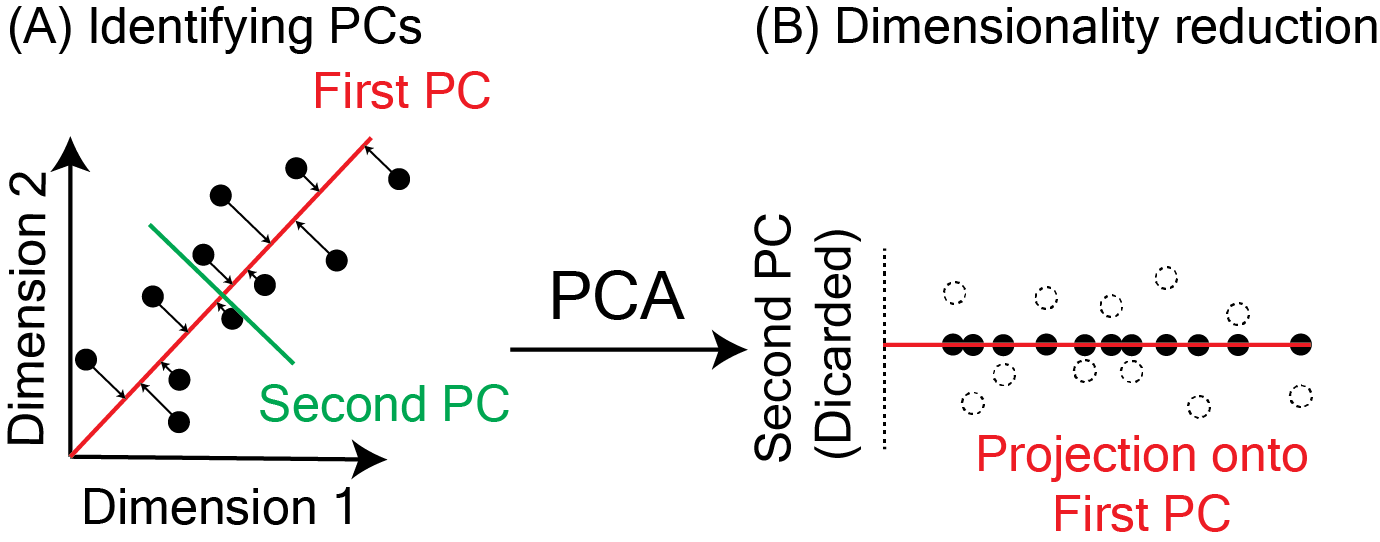
\includegraphics[width=\linewidth]{foundations/ch1/Images/pca_ex.png}
\caption[Principal components analysis]{\textbf{(A)} the observed data shown in the left scatter plot, where the points are two-dimensional. The first ``principal component'' (PC) is the axis in which the data varies the most, and the second PC is the axis (orthogonal to those of the preceding principal components) along which the data varies the second most. Projecting the data to the first PC is shown with the arrows. \textbf{(B)} the data is ``projected'' onto the first PC via PCA, by effectively ``reorienting'' the dataset along the first and second principal components (dashed circles and lines), and then removing the second PC entirely (solid circles) to reduce the dimensionality from two dimensions to one dimension. Think about this in a model-based manner, we ``discarded'' a direction in which the data varies less.}
\label{fig:ch1:pcaex}
\end{figure}

\newpage